%===========================================================
% This is the thesis template for the Statistics major at
% Amherst College. Brittney E. Bailey (bebailey@amherst.edu)
% adapted this template from the Reed College LaTeX thesis
% template in January 2019 with major updates in April 2020.
% Please send any comments/suggestions: bebailey@amherst.edu

% Most of the work for the original document class was done
% by Sam Noble (SN), as well as this template. Later comments
% etc. by Ben Salzberg (BTS). Additional restructuring and
% APA support by Jess Youngberg (JY). Email: cus@reed.edu
%===========================================================

\documentclass[12pt, twoside]{amherstthesis}
\usepackage{graphicx,latexsym}
\usepackage{amsmath}
\usepackage{amssymb,amsthm}
\usepackage{longtable,booktabs} %setspace loaded in .cls
\usepackage[hyphens]{url}
\usepackage{hyperref}
\usepackage{lmodern}
\usepackage{float}
\floatplacement{figure}{H}
\usepackage{rotating}
\usepackage{fancyvrb}
% User-added packages:
% End user-added packages

%===========================================================
% BIBLIOGRAPHY FORMATTING

% Next line commented out by CII
%%% \usepackage{natbib}
% Comment out the natbib line above and uncomment the
% following two lines to use the new biblatex-chicago style,
% for Chicago A. Also make some changes at the end where the
% bibliography is included.
%\usepackage{biblatex-chicago}
%\bibliography{thesis}


%===========================================================
% HYPERLINK FORMATTING

% Added by CII (Thanks, Hadley!)
% Use ref for internal links
\renewcommand{\hyperref}[2][???]{\autoref{#1}}
\def\chapterautorefname{Chapter}
\def\sectionautorefname{Section}
\def\subsectionautorefname{Subsection}
% End of CII addition
\usepackage{xcolor}
\hypersetup{
    colorlinks,
    linkcolor={red!50!black},
    citecolor={blue!50!black},
    urlcolor={blue!80!black}
}

%===========================================================
% CAPTION FORMATTING

% Added by CII
\usepackage{caption}
\captionsetup{width=5in}
% End of CII addition

%===========================================================
% TITLE FORMATTING

\renewcommand{\contentsname}{Table of Contents}

\usepackage{titlesec}
%%%%%%%%
% How to use titlesec:
% \titleformat{⟨command⟩}[⟨shape⟩]{⟨format⟩}{⟨label⟩}{⟨sep⟩}
%  {⟨before-code⟩}[⟨after-code⟩]
%%%%%%%%

\titleformat{\chapter}[hang]
{\normalfont%
    \Large% %change this size to your needs for the first line
    \bfseries}{\chaptertitlename\ \thechapter}{1em}{%
      %change this size to your needs for the second line
    }[]

\titleformat{\section}[hang]
{\normalfont%
    \large % %change this size to your needs for the first line
    \bfseries}{\thesection}{1em}{%
     %change this size to your needs for the second line
    }[]

\titleformat{\subsection}[hang]
{\normalfont%
    \normalsize % %change this size to your needs for the first line
    \bfseries}{\thesubsection}{1em}{%
     %change this size to your needs for the second line
    }[]

% \titleformat{\section}[display]
% {\normalfont%
%     \large% %change this size to your needs for the first line
%     \bfseries}{\chaptertitlename\ \thechapter}{20pt}{%
%     \normalsize %change this size to your needs for the second line
%     }


%===========================================================
% DOCUMENT FONT

% \usepackage{times}
% other fonts available eg: times, bookman, charter, palatino


%===========================================================
% PASSING FORMATS FROM RMD --> LATEX

%%%%%%%%
% NOTE: Dollar signs pass parameters between YAML inputs
% in index.Rmd and LaTeX
%%%%%%%%

\Abstract{
The abstract should be a short summary of your thesis work. A paragraph is usually sufficient here.
}

\Acknowledgments{
Use this space to thank those who have helped you in the thesis process (professors, staff, friends, family, etc.). If you had special funding to conduct your thesis work, that should be acknowledged here as well.
}

\Dedication{

}

\Preface{

}

% Formatting R code display
% Syntax highlighting #22

% Formatting R code: set baselinestretch = 1.5 for double-spacing
\DefineVerbatimEnvironment{Highlighting}{Verbatim}{
  baselinestretch = 1,
  commandchars=\\\{\}}

% Formatting R output display: set baselinestretch = 1.5 for double-spacing
\DefineVerbatimEnvironment{verbatim}{Verbatim}{
  baselinestretch = 1,
  % indent from left margin
  xleftmargin = 1mm,
  % vertical grey bar on left side of R output
  frame = leftline,
  framesep = 0pt,
  framerule = 1.5mm, rulecolor = \color{black!15}
  }

\title{My amazing title}
\author{Tony Ni}
\date{April DD, 20YY}
\division{}
\advisor{Brittney Bailey}
% for second advisor
\institution{Amherst College}
\degree{Bachelor of Arts}
\department{Mathematics and Statistics}

% Fix from pandoc about cslreferences?
% https://github.com/mpark/wg21/issues/54
\newlength{\cslhangindent}
\setlength{\cslhangindent}{1.5em}
\newenvironment{cslreferences}%
  {\setlength{\parindent}{0pt}%
  \everypar{\setlength{\hangindent}{\cslhangindent}}\ignorespaces}%
  {\par}

% Added by CII
%%% Copied from knitr
%% maxwidth is the original width if it's less than linewidth
%% otherwise use linewidth (to make sure the graphics do not exceed the margin)
\makeatletter
\def\maxwidth{ %
  \ifdim\Gin@nat@width>\linewidth
    \linewidth
  \else
    \Gin@nat@width
  \fi
}
\makeatother

% ===========================================
% DOCUMENT SPACING

\setlength{\parskip}{0pt}
% Added by CII

\providecommand{\tightlist}{%
  \setlength{\itemsep}{0pt}\setlength{\parskip}{0pt}}


% ===========================================
% ===========================================
% ===========================================
\begin{document}

\doublespace
% Everything below added by CII
  \maketitle

\frontmatter % this stuff will be roman-numbered
\pagenumbering{roman}
\pagestyle{fancyplain}
%\pagestyle{fancy} % this removes page numbers from the frontmatter

  \begin{abstract}
    The abstract should be a short summary of your thesis work. A paragraph is usually sufficient here.
  \end{abstract}
  \begin{acknowledgments}
    Use this space to thank those who have helped you in the thesis process (professors, staff, friends, family, etc.). If you had special funding to conduct your thesis work, that should be acknowledged here as well.
  \end{acknowledgments}

  \hypersetup{linkcolor=black}
  \setcounter{tocdepth}{2}
  \tableofcontents

  \addcontentsline{toc}{chapter}{List of Tables}\listoftables

  \addcontentsline{toc}{chapter}{List of Figures}\listoffigures


\mainmatter % here the regular arabic numbering starts
\pagenumbering{arabic}
\pagestyle{fancyplain} % turns page numbering back on

\hypertarget{intro}{%
\chapter{Introduction}\label{intro}}

\hypertarget{background}{%
\section{Background}\label{background}}

Coal is one of the most dangerous combustible fuels which is being burned in all across the world as one of the largest methods of obtaining energy. Yet, although it is a fossil fuel which is naturally abundant and easy to utilize, it is comprised of a long list of dangerous chemicals including -- but not limited to: arsenic, radium, boron, and a large list of other chemicals which prove to be dangerous to humans and animals alike. (Kelderman et al., 2019)

Power plants produce electricity by burning this coal, and as a result of how prevalent it is within the US - over 100 million tons of coal ash are produced every year. This side-product as a result of the coal combustion is often disposed by directly being dumped into landfills and waste ponds. (Kelderman et al., 2019)

Only recently have these complaints and lawsuits regarding the disposing practices made by non-profit environmental organizations been heard. Due to the onslaught of pressure put on the Environmental Protection Agency -- the Coal Ash Rule was bor in 2015. (Kelderman et al., 2019)

This rule has forced over 265 coal power plants -- about 3/4 of all coal power plants in the US - to make data regarding chemical concentrations publicly available to the general population. (Kelderman et al., 2019)

In their analysis using this data, the Environmental Integrity Project -- a non-profit organization dedicated to issues involving environmental justice have concluded that essentially all groundwater under coal plants are contaminated. (Kelderman et al., 2019)

However, is this really the case? There are many naturally occurring chemicals existing in groundwater as as such, perhaps their claims are overstated.
\begin{figure}

{\centering 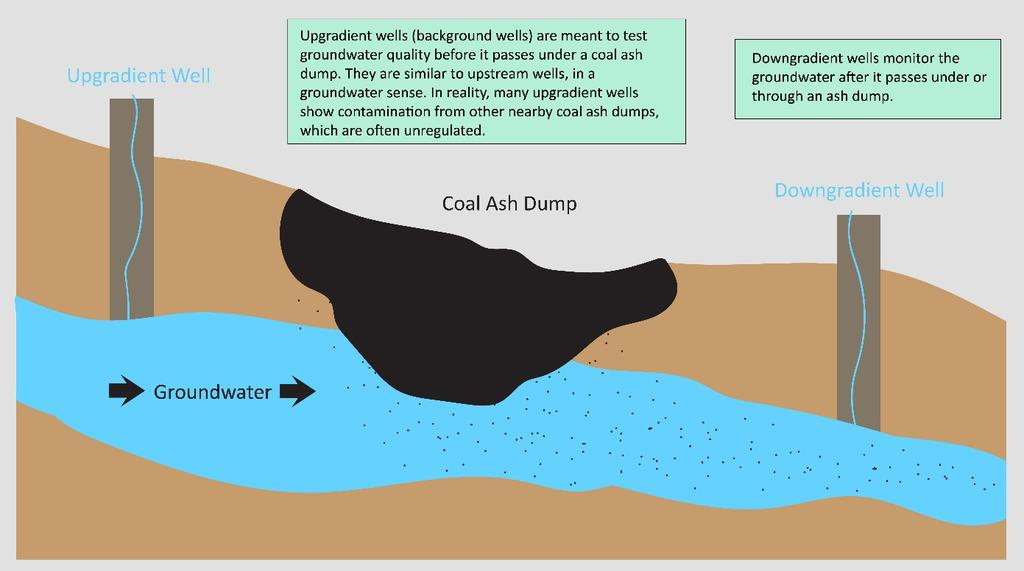
\includegraphics[width=1\linewidth]{figures/upgradientdowngradient} 

}

\caption{Difference Between Upgradient and Downgradient Wells}\label{fig:upgradientdowngradient}
\end{figure}
Typically in a coal ash plant, there exists two types of wells: upgradient wells and downgradient wells. These wells are essential to measure the amount of contamination being caused by coal ash. Upgradient wells, also known as background wells, measures the concentrations of chemicals in groundwater before it passes through an coal ash dump. Conversely, downgradient wells measure the concentrations of chemicals in groundwater after it passes through a coal ash dump.

With this information, typically -- one estimates the amount of chemical contamination caused by a coal as dump by subtracting the upgradient concentration from the downgradient concentration of a chemical (downgradient concentration - upgradient concentration).

However, due to the lack of proper reporting guidelines prior to the enactment of the Coal Ash Rule, we believe that there may be retired or even unregulated upgradient wells which can cause the concentrations of chemicals being recorded from these upgradient wells to be inaccurate or even completely wrong.

Our end goal remains the same as the EIP: to identify contaminated groundwater in coal plants -- but to attempt to find a way to effectively correct the improper/inaccurate values resulting from LOD errors and other factors which the EIP may not have considered.

The limit of detection problem stems from the measuring devices' inability to obtain chemical concentrations smaller than a certain threshold amount, thus affecting the measurements recorded.

Our plan is to utilize bootstrapping and imputation techniques to correct for these measurements by accounting for the innate contamination which may be caused by factors such as retired and unregulated wells that were mentioned before.

\hypertarget{data}{%
\section{Data}\label{data}}

\hypertarget{coalashrule}{%
\subsection{Coal Ash Rule}\label{coalashrule}}

A large coal ash spill at the Tennessee Valley Authority (TVA) which occured on December 22, 2008 in Kingston, TN -- prompted the Environmental Protection Agency (EPA) to propose a set of standardized regulations and procedures to address the concerns regarding coal ash plants nationwide in the US. (Environmental Protection Agency, 2020)

This was known as the Coal Ash Rule, passed on December 19, 2014. (Environmental Protection Agency, 2020)

Changes were made to the Coal Ash Rule over the years in the form of `amendments,' one of which made required facility information and data to be made publicaly available to the public (April 15, 2015 rule change) (Environmental Protection Agency, 2020)

\hypertarget{source-of-data}{%
\subsection{Source of Data}\label{source-of-data}}

The data used in the study are from the results published in ``Annual Groundwater Monitoring and Corrective Action Reports'' which were made available to the public in March 2018 as a result of the Coal Ash Rule. (Environmental Integrity Project, 2020)

These reports are in PDF format and are thousands of pages long, which makes it difficult for individuals to look through the data in a meaningful way. (Environmental Integrity Project, 2020)

The EIP obtained the data from an online, publicly available database containing groundwater monitoring results from the first ``Annual Groundwater Monitoring and Corrective Action Reports'' in 2018 which was collected from coal plants and coal ash dumps under the Coal Ash Rule (Environmental Integrity Project, 2020)

They wrangled the data into a more accessible machine-readable format which contains information from over 443 annual groundwater monitoring reports posted by 265 coal ash plants, which is downloadable from the EIP's website. (Environmental Integrity Project, 2020)

\newpage

\hypertarget{variables}{%
\subsection{Variables}\label{variables}}

The dataset contains information regarding chemical concentrations at coal plants. A coal plant consists of multiple disposal areas for the coal ash that it produces. At each disposal area, there are specific locations that groundwater is being measured, known as wells which represent an observation in the dataset. There are two types of wells -- upgradient and downgradient wells. The variables consist of information regarding the specific chemical concentrations of each well. From the 19 different contaminants (antimony, arsenic, boron, etc.) a major problem is that some wells only have measurements for certain chemicals and don't have them for others.

\hypertarget{plan-of-action}{%
\subsection{Plan of Action}\label{plan-of-action}}

Within the report, the EIP mentions certain restrictions within the data that have caused their data to potentially be inaccurate (specifically, with limit of detection problems, and a large amount of missing chemical data). The limit of detection problem comes when measuring devices used to measure chemical concentrations are unable to detect below a certain threshold, causing large numbers of observations to have duplicate, wrong values -- which can cause for misguided analysis.The other issue is less guided/formed, but for brevity, we think that a lot of the issues in the data comes from the potential possibility of contamination during data collection from investigators from non coal-ash sources. This may include things like: retired/unregulated wells which are old and have chemicals leaking into the groundwater, mismanagement in measuring, etc.My project hopes to work with methods on handling this missing data -- alongside investing potential uses of bootstrapping and other resampling methods (potentially?) in order to try to come up with a more statistically accurate and sound result by looking to assuage the problems that the EIP faced in their analysis. Specifically, to find a way to split up the data into ''uncontaminated'' and ''contaminated'' wells in order to find the natural distribution of chemicals in each -- and doing to so in the face of data corrupted by LOD problems and inaccuracies. I'm hoping to apply and compare different ways of altering the data to account for these myriad of issues in order to look for more salient findings that the EIP might have missed or if not, to see if improvements can be made regarding the way that contaminated coal ash wells are being identified.

\hypertarget{methodology}{%
\chapter{Methodology}\label{methodology}}

\hypertarget{planofaction}{%
\section{Plan of Action}\label{planofaction}}

\hypertarget{substitution}{%
\subsection{Substitution}\label{substitution}}

\hypertarget{corrections}{%
\chapter*{Corrections}\label{corrections}}
\addcontentsline{toc}{chapter}{Corrections}

A list of corrections after submission to department.

Corrections may be made to the body of the thesis, but every such correction will be acknowledged in a list under the heading ``Corrections,'' along with the statement ``When originally submitted, this honors thesis contained some errors which have been corrected in the current version. Here is a list of the errors that were corrected.'' This list will be given on a sheet or sheets to be appended to the thesis. Corrections to spelling, grammar, or typography may be acknowledged by a general statement such as ``30 spellings were corrected in various places in the thesis, and the notation for definite integral was changed in approximately 10 places.'' However, any correction that affects the meaning of a sentence or paragraph should be described in careful detail. The files samplethesis.tex and samplethesis.pdf show what the ``Corrections'' section should look like. Questions about what should appear in the ``Corrections'' should be directed to the Chair.

\backmatter

\hypertarget{references}{%
\chapter*{References}\label{references}}
\addcontentsline{toc}{chapter}{References}

\noindent

\setlength{\parindent}{-0.20in}
\setlength{\leftskip}{0.20in}
\setlength{\parskip}{8pt}

\hypertarget{refs}{}
\begin{cslreferences}
\leavevmode\hypertarget{ref-EIP2020}{}%
Environmental Integrity Project. (2020). Coal Ash Groundwater Contamination: Documenting Coal Ash Pollution. Retrieved from \url{https://environmentalintegrity.org/coal-ash-groundwater-contamination/}

\leavevmode\hypertarget{ref-Car2020}{}%
Environmental Protection Agency. (2020). Disposal of Coal Combustion Residuals from Electric Utilities Rulemakings. Retrieved from \url{https://www.epa.gov/coalash/coal-ash-rule}

\leavevmode\hypertarget{ref-Kelderman2019}{}%
Kelderman, K., Kunstman, B., Roy, H., Sivakumar, N., Mccormick, S., \& Bernhardt, C. (2019). Coal's Poisonous Legacy: Groundwater Contaminated by Coal Ash Across the U.S.
\end{cslreferences}
% Index?

\end{document}
